% !TEX program = pdflatex
\documentclass[11pt,a4paper]{article}
\usepackage[T1]{fontenc}
\usepackage[utf8]{inputenc}
\usepackage{lmodern}
\usepackage[italian]{babel}
\usepackage{amsmath,amssymb}
\usepackage{graphicx}
\usepackage{xcolor}
\usepackage[a4paper,margin=2.4cm]{geometry}
\usepackage{array}
\usepackage{float}
\usepackage{hyperref}
\providecommand{\micro}{}
\renewcommand{\micro}{\ensuremath{\mathrm{\mu}}}
\hypersetup{colorlinks=true,linkcolor=blue!55!black,citecolor=blue!55!black,
  urlcolor=blue!55!black,
  pdftitle={Motore Fotonico del Vuoto V7.2 - Appendice},
  pdfauthor={Francesco Bulla}}
\setlength{\parskip}{0.35em}
\setlength{\parindent}{1.2em}

\title{\bfseries Il costo del contrappeso, la finestra a 1064 nm\\
e la natura fisica del latch\\[0.3em]
\large Appendice V7.2 al Preprint V7.1}
\author{Francesco Bulla\\ \small Catania, Italia}
\date{29 ottobre 2026 \quad \small versione 7.2}

\begin{document}
\maketitle

\begin{abstract}
\noindent
La V7.2 chiude tre questioni che la V7.1 aveva lasciato aperte: il costo
energetico del contrappeso, la finestra termica a 1064 nm e la natura fisica
del latch. Il risultato principale è che il ciclo di 720$^\circ$ non è una
firma dell'orientazione. L'orientazione resta periodica di 360$^\circ$; il
subarmonico a $f_{\rm rot}/2$ appartiene allo \emph{stato del collegamento},
che è dispari sotto 360$^\circ$. Il contrappeso costa un fattore 2.44 a metà
ciclo e 3.88 nel limite conservativo, a pari angolo; rispetto a un ciclo
banale di 360$^\circ$ il latch a metà costa 4.88, il limite conservativo
7.76. La modulazione di $\omega$ è 74.2\,\%,
non 84.2\,\%: l'84.2\,\% è la frazione di inerzia e conta solo nel transitorio
(nanosecondi). A 1064 nm la profondità balistica passa da 22 a 28\,$\micro$m e
il buco termico a 2.3\,$\micro$m si chiude, ma il bordo a basso $R$ resta
termico: 1064 nm non sposta la soglia di potenza a $R=0.3\,\micro$m. La soglia
di 20\,K non è una soglia di sicurezza biologica (57\,$^\circ$C); la soglia
prudente è 5\,K (42\,$^\circ$C). Il latch è un vincolo reversibile, non un
cavo: senza un meccanismo fisico misurato il modello resta cinematico.
\end{abstract}

\section*{Sintesi in sei righe}
\addcontentsline{toc}{section}{Sintesi in sei righe}
\begin{enumerate}\itemsep2pt
\item \textbf{Il prezzo del contrappeso.} $I$ cresce di 6.31, $\beta$ di
3.88. A regime $\omega=\tau/\beta$: quando il contrappeso è innestato il
rallentamento è 3.88, non 6.31; sul ciclo a metà il fattore è 2.44.
L'inerzia conta nel transitorio $\tau_{\rm spin}=I/\beta\approx 7$\,ns.
\item \textbf{Il costo dei 720$^\circ$.} Con il latch a metà ciclo
$T_{720}=T_{360}^{\rm no}+T_{360}^{\rm cw}$: 2.44 volte un 720$^\circ$ senza
contrappeso, 4.88 volte un 360$^\circ$ senza. Il 3.88 della V7.1 è il limite
conservativo con contrappeso sempre innestato.
\item \textbf{La firma.} $\omega$ modula a $f_{\rm rot}$; lo stato A/B modula
a $f_{\rm rot}/2$. Il subarmonico a $\omega/2$ esiste solo in un osservabile
dispari sotto 360$^\circ$.
\item \textbf{1064 nm.} La profondità passa da 22 a 28\,$\micro$m; il buco a
2.34\,$\micro$m si sposta a 3.11\,$\micro$m e scende sotto 20\,K. A
$R=0.3\,\micro$m $P_{\rm target}$ cresce con $\lambda$: la finestra a basso
$R$ non si allarga.
\item \textbf{Il rumore.} A $Pe_r=10$ la diffusione rotazionale sparpaglia
l'orientazione di $\sim 80^\circ$ per giro. Con il segnale di orientazione lo
stato 720$^\circ$ si ripiega in 10 cicli; l'FFT cieca richiede 100--600 cicli.
\item \textbf{Il latch.} È un linker reversibile (spot ottico, DNA, bead
magnetica), non un cavo. Il modello non dimostra che esista: calcola quanto
costerebbe e come si falsificherebbe.
\end{enumerate}

\section{Tre correzioni alla V7.1}
\label{sec:correzioni}

Prima di aggiungere qualunque cosa, la V7.1 va corretta in tre punti. Non
sono dettagli: cambiano le conclusioni.

\subsection{La modulazione è 74.2\,\%, non 84.2\,\%}

La V7.1 calcolava
\begin{equation}
m_I = 1-\frac{I_{\rm rot}}{I_{\rm tot}} = 0.8416
\end{equation}
e la chiamava ``modulazione di $\omega$''. Non lo è. A regime la velocità è
$\omega=\tau/\beta_{\rm tot}$; la modulazione è
\begin{equation}
m_\omega = 1-\frac{\beta_{\rm rot}}{\beta_{\rm tot}} = 0.7423.
\label{eq:modomega}
\end{equation}
L'84.2\,\% è la frazione di inerzia: dice quanto pesa il contrappeso
nell'avvio, non quanto rallenta il regime. Il transitorio è
$\tau_{\rm spin}=I_{\rm tot}/\beta_{\rm tot}\approx 6.6$\,ns a
$R=0.3\,\micro$m, contro $T_{360}\approx 1.5$\,s: sei ordini di grandezza
sotto. La figura della V7.1 va rifatta con 74.2\,\%.

\subsection{Il fattore 3.88 è il limite conservativo, non il caso fisico}

La V7.1 calcolava $T_{720}=2T_{360}^{\rm cw}$, cioè assumeva il contrappeso
innestato per tutti i 720$^\circ$. L'idea dice che il latch si attiva
\emph{dopo} 360$^\circ$. Il caso fisico è quindi
\begin{equation}
T_{720}^{1/2}=T_{360}^{\rm no}+T_{360}^{\rm cw}
=\frac{2\pi(\beta_{\rm no}+\beta_{\rm cw})}{\tau},
\label{eq:t720half}
\end{equation}
mentre il limite conservativo resta
\begin{equation}
T_{720}^{\rm full}=\frac{4\pi\beta_{\rm cw}}{\tau}.
\label{eq:t720full}
\end{equation}
Con $\beta_{\rm cw}=3.881\beta_{\rm no}$:
\begin{equation}
\frac{T_{720}^{1/2}}{T_{720}^{\rm no}}=2.4406,\qquad
\frac{T_{720}^{\rm full}}{T_{720}^{\rm no}}=3.8811.
\end{equation}
Rispetto a un \emph{singolo} 360$^\circ$ senza contrappeso, i fattori sono
4.881 e 7.762. La frase ``il 720 costa il 288\,\% in più'' è vera solo nel
limite conservativo e solo a pari angolo; rispetto a un 360$^\circ$ costa il
676\,\%. Va scritto con il caso accanto.

\subsection{Il subarmonico è nello stato, non nell'orientazione}

L'orientazione $\theta(t)$ è periodica di 360$^\circ$: dopo un giro il corpo
è tornato. La velocità $\omega(t)$ è modulata una volta per giro, quindi il
suo spettro ha una riga a $f_{\rm rot}$, non a $f_{\rm rot}/2$. Il periodo di
720$^\circ$ appartiene allo \emph{stato del collegamento}: se A e B si
scambiano a 360$^\circ$ e tornano a 720$^\circ$, l'osservabile
$s(\theta)$ che legge A/B è dispari sotto 360$^\circ$,
$s(\theta+2\pi)=-s(\theta)$, e ha periodo $4\pi$. Solo questo osservabile ha
il subarmonico a $f_{\rm rot}/2$. La Figura~\ref{fig:firma}
va letta così: la curva di $\omega$ e quella di A/B hanno periodi diversi.

\section{Il costo energetico del contrappeso}
\label{sec:costo}

\subsection{Le equazioni}

Sia $\tau=Pe_r kT$ la coppia richiesta, fissata dal criterio $Pe_r=10$. La
potenza al bersaglio è
\begin{equation}
P_{\rm target}=\frac{Pe_r kT}{\tau/P},
\label{eq:ptarget}
\end{equation}
dove $\tau/P$ dipende da $R$, $\lambda$ e dal ritardo $\delta$, non da
$\beta$. Quindi $P_{\rm inc}=P_{\rm target}/T_s(z)$ è la stessa con o senza
contrappeso, a parità di $R$, $\lambda$ e $z$. L'energia depositata in un
ciclo è
\begin{equation}
E=P_{\rm inc}T.
\label{eq:energia}
\end{equation}
Poiché $P_{\rm inc}$ non cambia, $E$ scala con $T$, cioè con $\beta$.

\subsection{I numeri}

La Tabella~\ref{tab:costo} riporta i tre casi. A $R=1\,\micro$m il ciclo
senza contrappeso dura 29.52\,s; con il latch a metà 72.04\,s; con il
contrappeso sempre innestato 114.56\,s. L'energia passa da 0.87 a 4.23 a
6.73\,mJ. Il rapporto 2.44 è il caso fisico; il 3.88 è il limite
conservativo.

\begin{table}[H]
\centering\small
\begin{tabular}{rrrrrrrrrr}
\hline
$R$ & $T_{360}^{\rm no}$ & $T_{720}^{\rm no}$ & $T_{720}^{1/2}$ &
$T_{720}^{\rm full}$ & $E_{360}^{\rm no}$ & $E_{720}^{1/2}$ &
$E_{720}^{\rm full}$ & $\frac{E_{720}^{1/2}}{E_{720}^{\rm no}}$ &
$\frac{E_{720}^{\rm full}}{E_{720}^{\rm no}}$ \\
\micro m & s & s & s & s & mJ & mJ & mJ & -- & -- \\
\hline
0.3 & 0.40 & 0.80 & 1.94 & 3.09 & 0.28 & 1.37 & 2.18 & 2.44 & 3.88 \\
0.5 & 1.84 & 3.69 & 9.00 & 14.32 & 0.31 & 1.50 & 2.38 & 2.44 & 3.88 \\
1.0 & 14.76 & 29.52 & 72.04 & 114.56 & 0.87 & 4.23 & 6.73 & 2.44 & 3.88 \\
2.0 & 118.07 & 236.13 & 576.29 & 916.45 & 29.45 & 143.74 & 228.58 & 2.44 & 3.88 \\
\hline
\end{tabular}

\caption{Costo energetico del contrappeso a 800\,nm, $z=2\,\micro$m,
$Pe_r=10$. Le ultime due colonne sono i rapporti rispetto a un ciclo di
720$^\circ$ senza contrappeso.}
\label{tab:costo}
\end{table}

\subsection{La frase da scrivere nel preprint}

\begin{quote}
Innestare il contrappeso moltiplica l'inerzia di 6.31 e l'attrito di 3.88.
A parità di $Pe_r$, la potenza al bersaglio non dipende da $\beta$:
$P_{\rm target}=Pe_r kT/(\tau/P)$ e $\tau/P$ dipende solo da $R$, $\lambda$ e
$\delta$. Quindi la potenza assorbita è la stessa con o senza contrappeso.
Ma il ciclo dura di più. Nel limite conservativo della V7.1, con il
contrappeso innestato per tutti i 720$^\circ$, $T_{720}$ cresce di 3.88 e
$E_{720}$ di 3.88. Con il latch a metà ciclo, che è il caso fisico,
$T_{720}$ cresce di 2.44 rispetto a un 720$^\circ$ senza contrappeso e di
4.88 rispetto a un 360$^\circ$ senza. La topologia SU(2) costa quindi il
144\,\% in più a pari angolo (o il 288\,\% nel limite conservativo); rispetto
a un ciclo banale di 360$^\circ$, il latch a metà costa il 388\,\% e il
limite conservativo il 676\,\%. Se l'obiettivo è
minimizzare il danno termico, il contrappeso è svantaggioso. Se l'obiettivo è
misurare la topologia, il costo è il prezzo dell'informazione topologica.
\end{quote}

L'aumento di inerzia non è la causa del rallentamento: a regime
$\omega=\tau/\beta$. L'inerzia entra solo in $\tau_{\rm spin}=I/\beta$, che a
$R=0.3\,\micro$m vale $6.6$\,ns. Il contrappeso rallenta perché aggiunge
attrito, non perché aggiunge massa.

\begin{figure}[H]
\centering
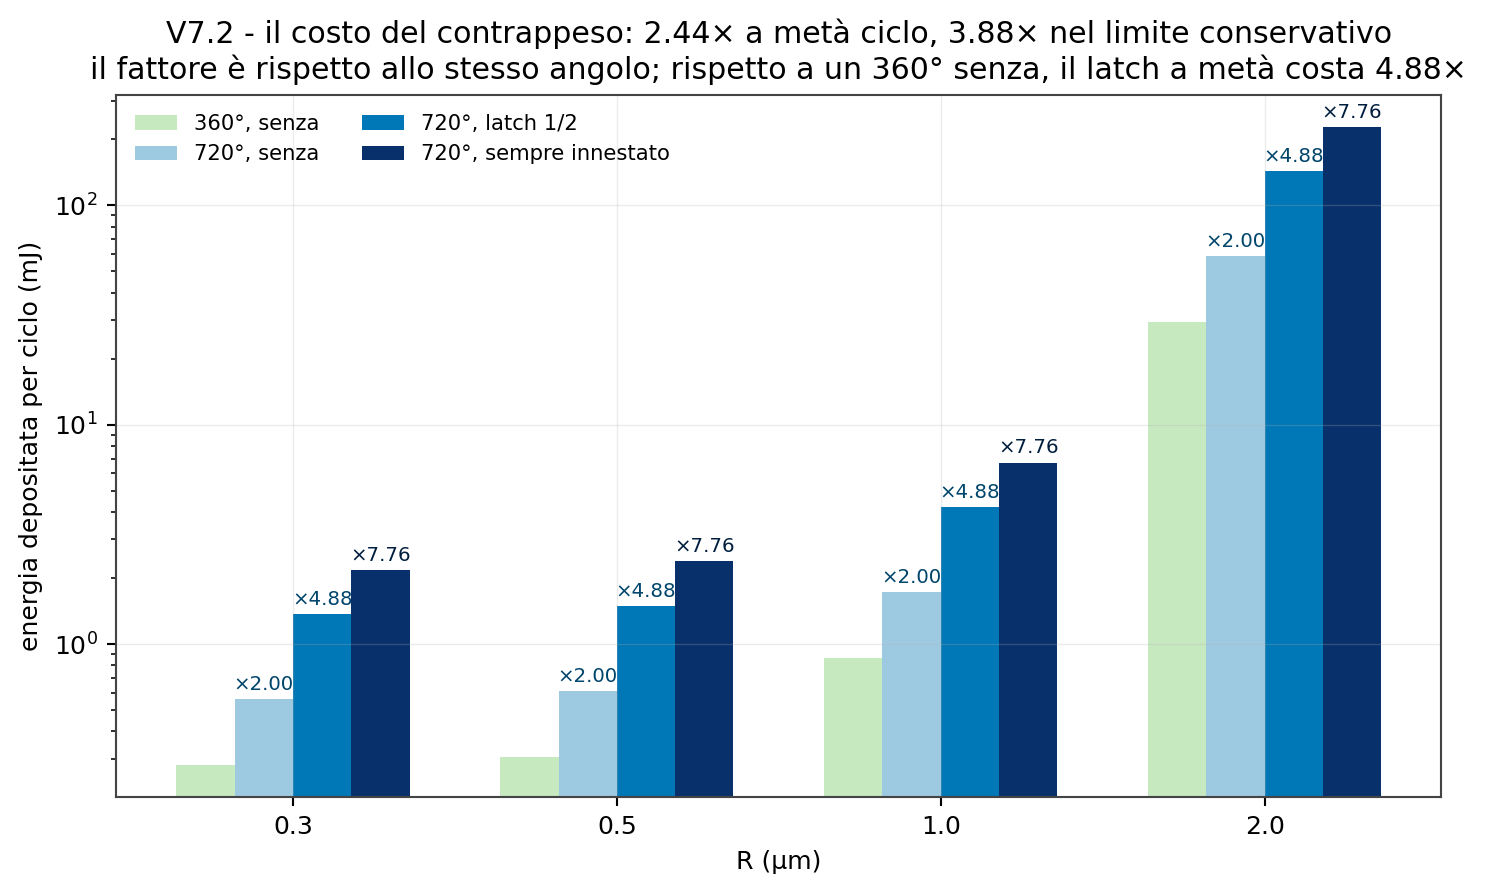
\includegraphics[width=\textwidth]{../figure/fig_V72_contrappeso.png}
\caption{Energia per ciclo a 800\,nm, $z=2\,\micro$m. Le etichette sono
rapporti rispetto al ciclo di 360$^\circ$ senza contrappeso; il testo usa i
rapporti a pari angolo (2.44 e 3.88).}
\label{fig:costo}
\end{figure}

\section{1064 nm: cosa cambia davvero}
\label{sec:1064}

\subsection{La profondità}

La Tabella~\ref{tab:lambda} e la Figura~\ref{fig:profondita} riportano i
numeri. A 1064\,nm $\mu_a$ scende da 430 a 200\,m$^{-1}$, ma $\mu_s$ scende
solo da 450 a 350\,cm$^{-1}$: la profondità balistica passa da 22.0 a
28.4\,$\micro$m, non a millimetri. A $z=2\,\micro$m la trasmissione passa da
0.913 a 0.932 (guadagno del 2\,\%); a $z=10\,\micro$m da 0.635 a 0.703
(guadagno dell'11\,\%). Il guadagno è reale ma modesto, perché nello scattering
il sangue resta dominato dai globuli rossi.

\begin{table}[H]
\centering\small
\begin{tabular}{rrrrrrrrl}
\hline
$R$ & $\lambda$ & $P_{\rm target}$ & $P_{\rm inc}$ & $\delta$ &
$\Delta T$ & $T_{720}$ & $E_{720}$ & sicuro \\
\micro m & nm & \micro W & mW & rad & K & s & mJ & \\
\hline
0.3 & 532 & 459 & 0.55 & 1.20 & 17.6 & 1.94 & 1.1 & solo op. \\
0.3 & 800 & 644 & 0.71 & 0.80 & 12.3 & 1.94 & 1.4 & solo op. \\
0.3 & 1064 & 836 & 0.90 & 0.60 & 12.2 & 1.94 & 1.7 & solo op. \\
0.5 & 532 & 123 & 0.15 & 2.01 & 4.7 & 9.00 & 1.3 & sì \\
0.5 & 800 & 152 & 0.17 & 1.34 & 2.9 & 9.00 & 1.5 & sì \\
0.5 & 1064 & 189 & 0.20 & 1.00 & 2.8 & 9.00 & 1.8 & sì \\
1.0 & 532 & 93 & 0.11 & 4.02 & 3.6 & 72.04 & 8.0 & sì \\
1.0 & 800 & 54 & 0.06 & 2.67 & 1.0 & 72.04 & 4.2 & sì \\
1.0 & 1064 & 53 & 0.06 & 2.01 & 0.8 & 72.04 & 4.1 & sì \\
2.0 & 532 & 131 & 0.16 & 8.03 & 5.0 & 576.29 & 90.0 & solo op. \\
2.0 & 800 & 228 & 0.25 & 5.34 & 4.3 & 576.29 & 143.7 & sì \\
2.0 & 1064 & 47 & 0.05 & 4.02 & 0.7 & 576.29 & 28.9 & sì \\
5.0 & 532 & 176 & 0.21 & 20.08 & 6.7 & 9004.56 & 1883.8 & solo op. \\
5.0 & 800 & 201 & 0.22 & 13.35 & 3.8 & 9004.56 & 1977.9 & sì \\
5.0 & 1064 & 45 & 0.05 & 10.04 & 0.7 & 9004.56 & 437.2 & sì \\
\hline
\end{tabular}

\caption{Confronto 532/800/1064\,nm a $z=2\,\micro$m, latch a metà ciclo.
``solo op.'' significa $5<\Delta T<20$\,K: valido per il criterio operativo
della V7.1, non prudente.}
\label{tab:lambda}
\end{table}

\begin{figure}[H]
\centering
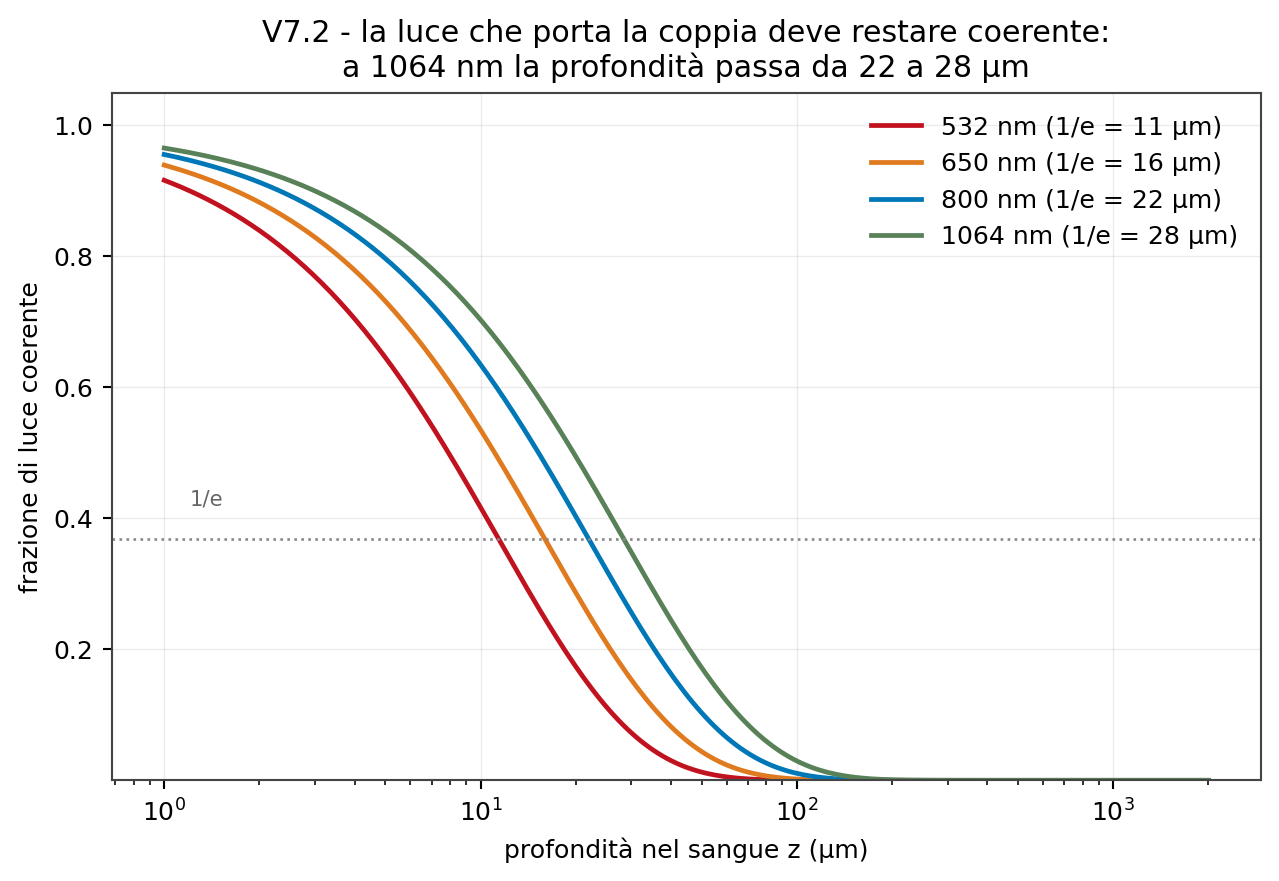
\includegraphics[width=0.78\textwidth]{../figure/fig_V72_profondita.png}
\caption{Frazione di luce coerente nel sangue intero. A 1064\,nm la
profondità 1/e è 28.4\,$\micro$m.}
\label{fig:profondita}
\end{figure}

\subsection{Perché a $R=0.3\,\micro$m 1064 nm non aiuta}

A piccolo $R$ il ritardo è piccolo, $\delta\propto 1/\lambda$,
$c_{\rm circ}=\langle1-\cos\delta\rangle\propto\delta^2\propto1/\lambda^2$,
mentre la coppia per fotone cresce come $\lambda$. Il risultato netto è
$\tau/P\propto1/\lambda$, quindi $P_{\rm target}\propto\lambda$:
644\,$\micro$W a 800\,nm, 836\,$\micro$W a 1064\,nm. Il maggiore assorbimento
dell'acqua a 1064 compensa quasi esattamente il minore assorbimento
dell'emoglobina: $\Delta T$ a $R=0.3\,\micro$m è 12.3\,K a 800\,nm e 12.2\,K
a 1064\,nm. Il bordo a basso $R$ è fissato dalla forma di ritardo, non dalla
trasparenza del sangue.

\subsection{Perché a $R\ge1\,\micro$m 1064 nm aiuta}

A $R\ge1\,\micro$m $\delta$ si avvicina a $\pi$ e la forma di ritardo non è
più Rayleigh. A $R=1\,\micro$m $\Delta T$ scende da 1.0 a 0.8\,K; a
$R=2\,\micro$m da 4.3 a 0.7\,K; a $R=5\,\micro$m da 3.8 a 0.7\,K. Il buco
termico a 2.34\,$\micro$m, dove $c_{\rm circ}$ si annulla, si sposta a
3.11\,$\micro$m e scende da 27.2 a 15.7\,K, sotto il limite di 20\,K. La
Figura~\ref{fig:ciclo} mostra l'effetto.

\begin{figure}[H]
\centering
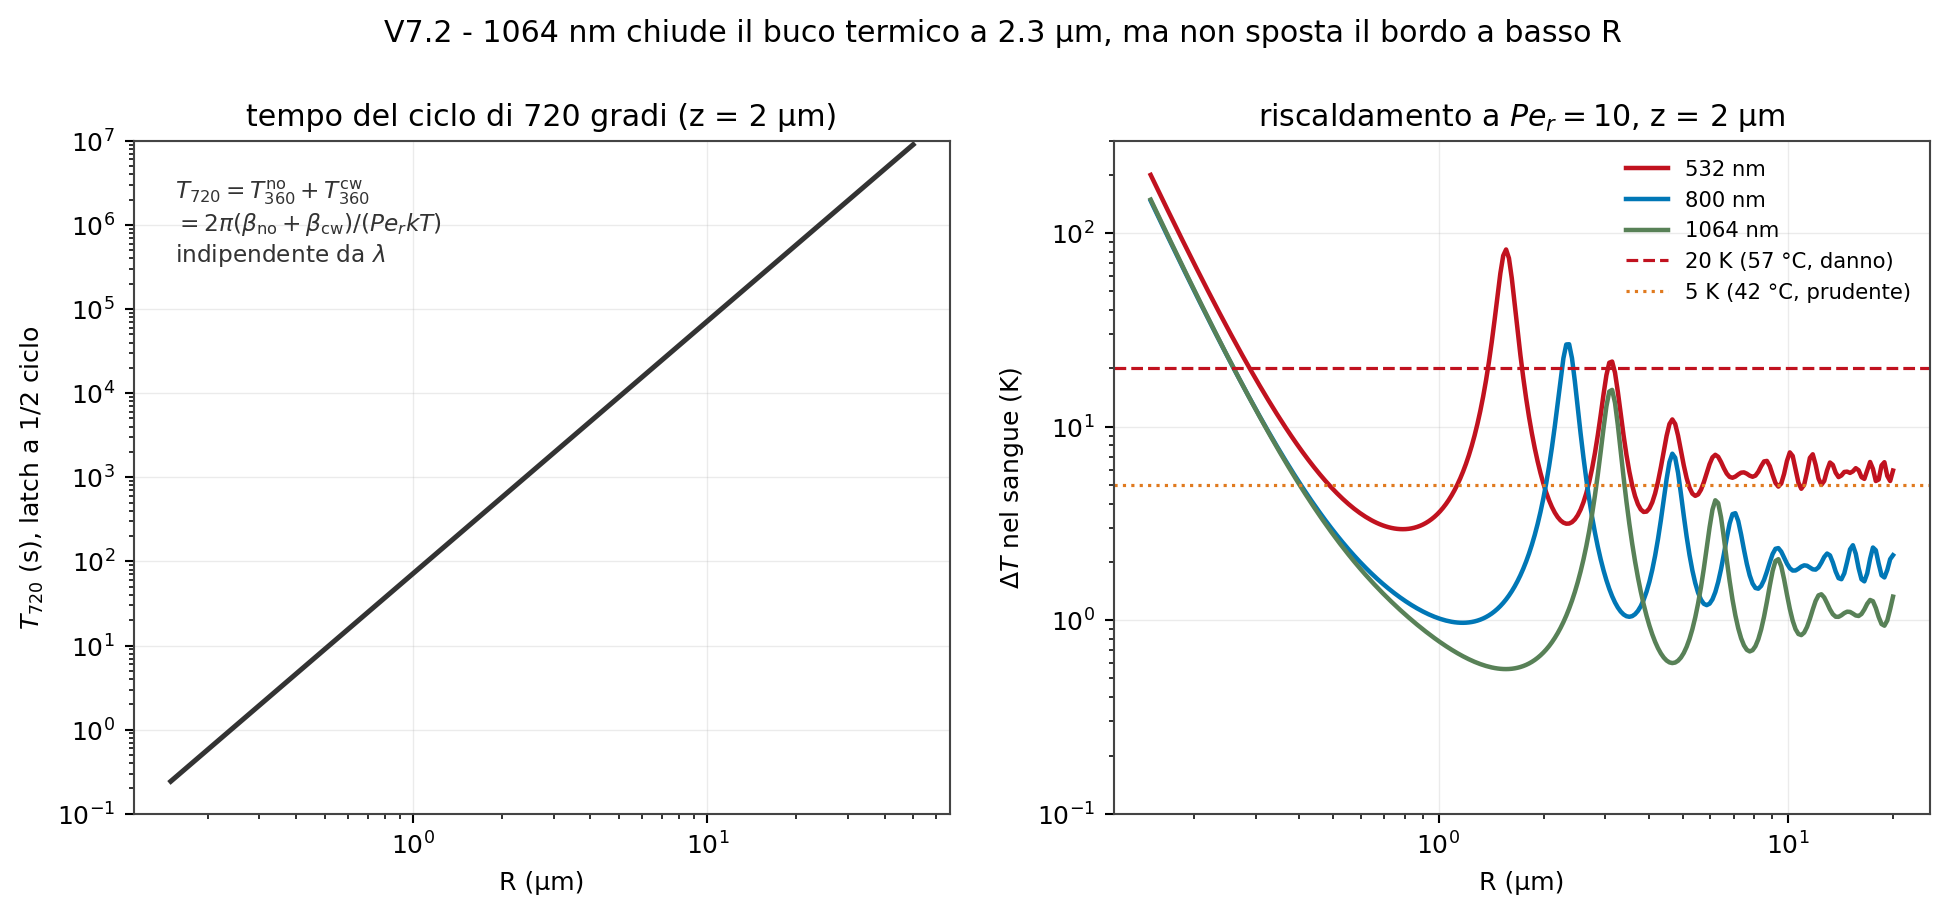
\includegraphics[width=\textwidth]{../figure/fig_V72_ciclo.png}
\caption{A sinistra il tempo del ciclo (indipendente da $\lambda$); a destra
il riscaldamento. Il picco a 2.34\,$\micro$m di 800\,nm è lo zero di
$\langle1-\cos\delta\rangle$; a 1064\,nm lo zero si sposta a 3.11\,$\micro$m
e resta sotto 20\,K.}
\label{fig:ciclo}
\end{figure}

\subsection{I picchi non sono risonanze Mie del modello}

I picchi di $\Delta T$ versus $R$ sono zeri di
$c_{\rm circ}=\langle1-\cos\delta\rangle$ a $\delta=2\pi m$. Per una sfera,
$\delta=2\pi\Delta n(2R)/\lambda$, quindi
\begin{equation}
R_m=\frac{m\lambda}{2\Delta n}.
\label{eq:zeri}
\end{equation}
A 532\,nm: 1.55, 3.11, 4.69\,$\micro$m. A 800\,nm: 2.34, 4.69\,$\micro$m. A
1064\,nm: 3.11, 6.23\,$\micro$m. Sono zeri della forma di ritardo, non
risonanze morfologiche di Mie. Una trattazione Mie completa aggiunge le
risonanze morfologiche; la dispersione di taglia smorza gli zeri. La
Tabella~\ref{tab:dispersione} mostra l'effetto: a 800\,nm e
$R=2.34\,\micro$m, $\Delta T$ passa da 27.2\,K con dispersione del 10\,\% a
12.5\,K con 15\,\% e 7.3\,K con 20\,\%. Il buco termico è un artefatto di
monodispersità, non una proprietà del sangue. La predizione è falsificabile:
misurare la distribuzione di taglia del campione. Se il CV è $\ge15\,\%$, il
picco a 2.34\,$\micro$m non deve superare 20\,K.

\begin{table}[H]
\centering\small
\begin{tabular}{rrrrr}
\hline
$\lambda$ & $R$ & dispersione & $P_{\rm target}$ & $\Delta T$ \\
nm & \micro m & \% & \micro W & K \\
\hline
800 & 2.34 & 10 & 1427 & 27.2 \\
800 & 2.34 & 15 & 654 & 12.5 \\
800 & 2.34 & 20 & 383 & 7.3 \\
800 & 2.34 & 30 & 190 & 3.6 \\
1064 & 3.11 & 10 & 1072 & 15.7 \\
1064 & 3.11 & 15 & 492 & 7.2 \\
1064 & 3.11 & 20 & 288 & 4.2 \\
1064 & 3.11 & 30 & 143 & 2.1 \\
532 & 1.55 & 10 & 2130 & 81.7 \\
532 & 1.55 & 15 & 985 & 37.8 \\
532 & 1.55 & 20 & 578 & 22.2 \\
532 & 1.55 & 30 & 287 & 11.0 \\
\hline
\end{tabular}

\caption{Effetto della dispersione di taglia sugli zeri della forma di
ritardo, a $z=2\,\micro$m.}
\label{tab:dispersione}
\end{table}

\subsection{La finestra, e la soglia sbagliata}

La Tabella~\ref{tab:finestre} riporta le finestre su una griglia fitta. A
$z=2\,\micro$m, 800\,nm è valido su $0.27$--$2.12$ e $2.45$--$50\,\micro$m;
1064\,nm è valido su $0.27$--$50\,\micro$m. A $z=10\,\micro$m, 800\,nm è
valido su $0.36$--$1.97$ e $2.64$--$50\,\micro$m; 1064\,nm su
$0.36$--$2.84$ e $3.54$--$50\,\micro$m. Il bordo a basso $R$ è $0.27$ per
entrambi: è termico, non ottico. 1064\,nm non lo sposta.

La soglia di 20\,K è 57\,$^\circ$C: coagulazione. La soglia prudente per
esposizione prolungata è 5\,K, cioè 42\,$^\circ$C. A 5\,K il punto sicuro più
veloce è $R\approx0.5$--$0.6\,\micro$m, $T_{720}\approx7$--$12$\,s,
$E_{720}\approx1.4$--$1.8$\,mJ. Il punto ``più veloce'' della
V7.1, $R\approx0.26$--$0.28\,\micro$m con $\Delta T\approx19$\,K, non è un punto
operativo: è il bordo del danno termico.

\begin{table}[H]
\centering\scriptsize
\begin{tabular}{rrp{4.2cm}p{4.2cm}r}
\hline
$\lambda$ & $z$ & valido ($\Delta T<20$ K) & sicuro ($\Delta T<5$ K) &
$\max \Delta T$ \\
nm & \micro m & \micro m & \micro m & K \\
\hline
532 & 2 & 0.29--1.36; 1.83--2.84; 3.29--50.00 & 0.49--1.09; 2.12--2.64; 3.81--4.10; 5.51--5.51 & 19.4 \\
532 & 5 & 0.36--1.27; 1.83--2.84; 3.54--50.00 & -- & 20.0 \\
532 & 10 & 0.45--1.18; 1.97--2.64; 3.54--4.10; 5.12--5.93; 6.87--7.95; 9.21--9.21; 10.67--10.67; 12.37--12.37; 14.32--23.97; 27.76--50.00 & -- & 19.5 \\
532 & 15 & -- & -- & -- \\
532 & 20 & -- & -- & -- \\
800 & 2 & 0.27--2.12; 2.45--50.00 & 0.42--1.97; 2.84--4.42; 5.12--50.00 & 17.6 \\
800 & 5 & 0.31--2.12; 2.64--50.00 & 0.52--1.83; 2.84--4.10; 5.51--6.38; 7.39--50.00 & 19.1 \\
800 & 10 & 0.36--1.97; 2.64--50.00 & 0.65--1.70; 3.06--4.10; 5.51--6.38; 7.95--8.56; 10.67--11.49; 14.32--14.32; 16.59--16.59; 19.22--20.69; 29.88--32.16; 37.26--40.10 & 18.2 \\
800 & 15 & 0.39--1.97; 2.64--4.42; 5.12--50.00 & 0.76--1.58; 3.29--3.81; 5.51--5.93 & 18.8 \\
800 & 20 & 0.42--1.97; 2.84--4.42; 5.12--50.00 & 0.88--1.47; 3.29--3.81; 5.93--5.93 & 18.6 \\
1064 & 2 & 0.27--50.00 & 0.42--2.64; 3.54--50.00 & 17.4 \\
1064 & 5 & 0.31--2.84; 3.29--50.00 & 0.52--2.64; 3.81--5.93; 6.87--50.00 & 18.7 \\
1064 & 10 & 0.36--2.84; 3.54--50.00 & 0.61--2.45; 3.81--5.51; 6.87--8.56; 9.92--50.00 & 16.8 \\
1064 & 15 & 0.39--2.84; 3.54--50.00 & 0.65--2.45; 3.81--5.51; 6.87--8.56; 9.92--50.00 & 16.8 \\
1064 & 20 & 0.42--2.84; 3.54--50.00 & 0.76--2.28; 4.10--5.51; 7.39--8.56; 10.67--11.49; 13.31--50.00 & 19.5 \\
\hline
\end{tabular}

\caption{Finestre termiche su griglia fitta. ``valido'' è
$\Delta T<20$\,K; ``sicuro'' è $\Delta T<5$\,K.}
\label{tab:finestre}
\end{table}

\begin{figure}[H]
\centering
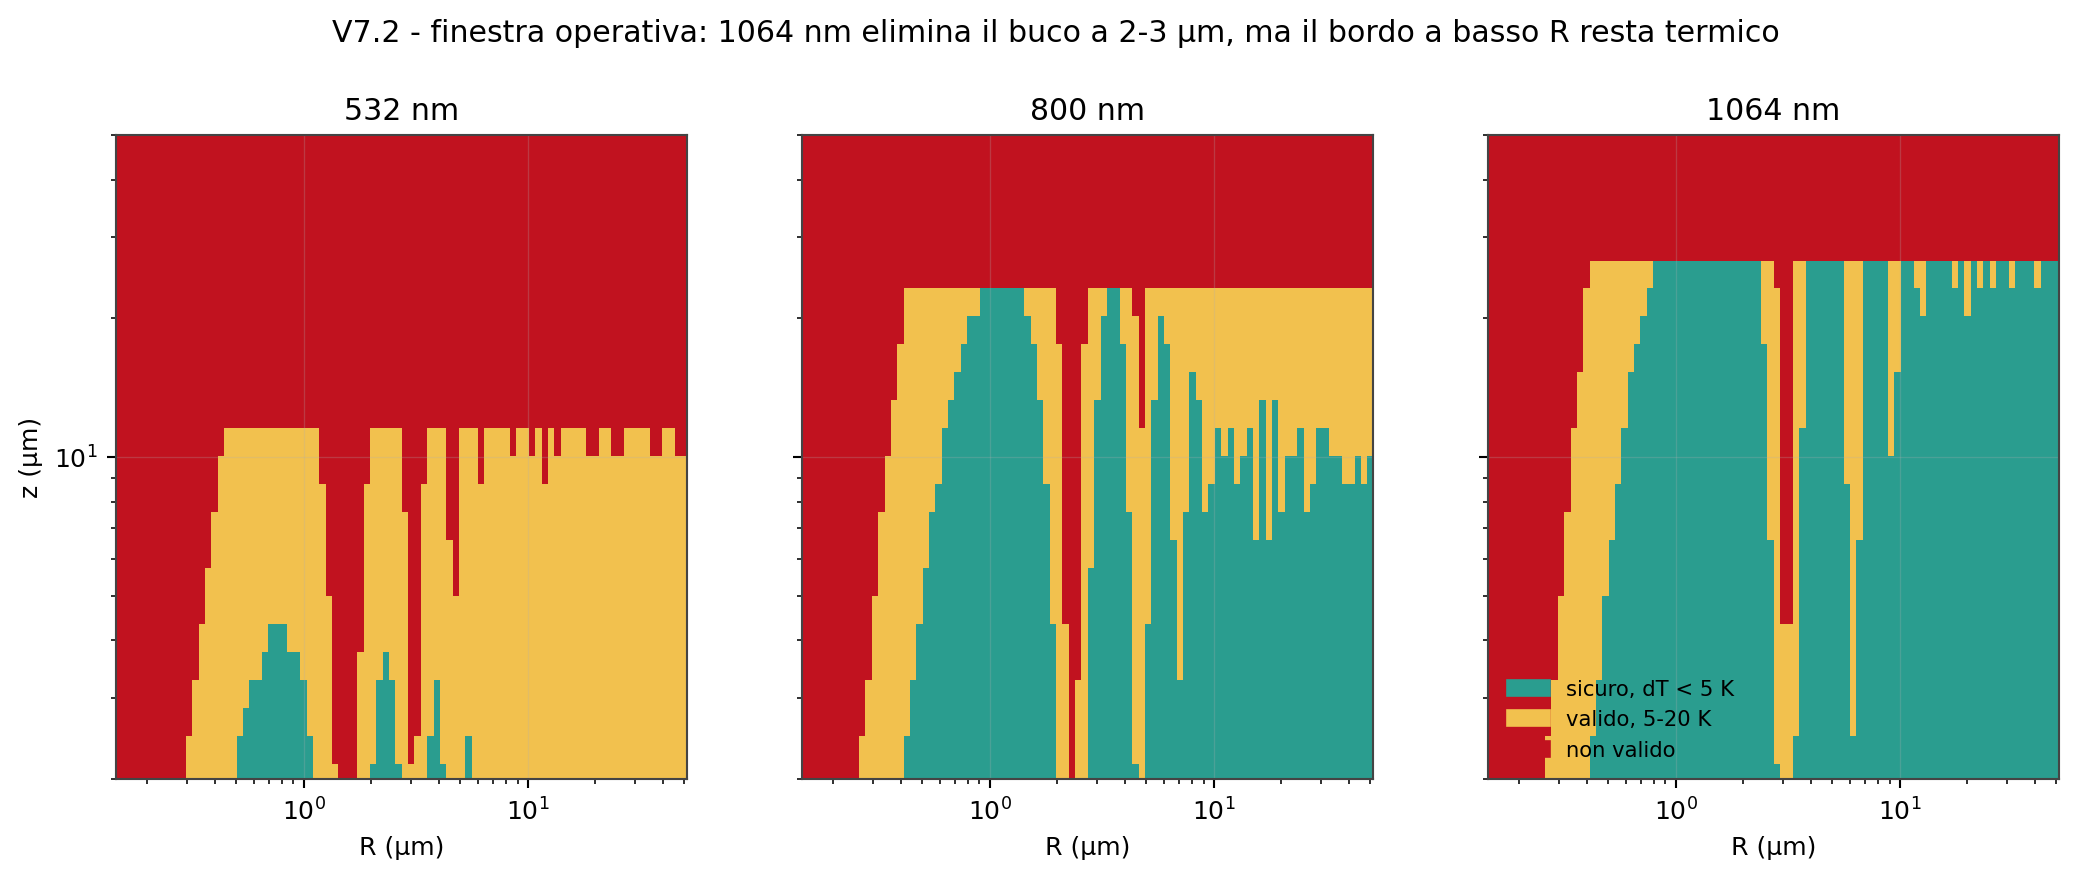
\includegraphics[width=\textwidth]{../figure/fig_V72_finestre.png}
\caption{Mappa $R$--$z$: verde sicuro ($\Delta T<5$\,K), giallo valido
($5$--$20$\,K), rosso non valido. 1064\,nm elimina il buco a
$2$--$3\,\micro$m, ma il bordo a basso $R$ resta rosso.}
\label{fig:finestre}
\end{figure}

\section{La natura fisica del latch}
\label{sec:latch}

\subsection{Cosa sono braccio, contrappeso e latch}

Il modello della V7.1 usava tre oggetti. Il primo è il \emph{braccio}: un
linker di lunghezza $d=2R$. A $R=0.3\,\micro$m è lungo $0.6\,\micro$m, non
una bacchetta macroscopica: è un vincolo molecolare (DNA origami, PEG rigido,
tether ottico). Il secondo è il \emph{contrappeso}: una bead di volume $V/2$,
cioè $r_{\rm cw}=0.794R=0.238\,\micro$m a $R=0.3\,\micro$m, alla distanza
$d=2R$. Non è un peso meccanico: è un secondo corpo idrodinamicamente
accoppiato. Il terzo è il \emph{latch}: un vincolo reversibile che si chiude
e si apre una volta per giro. Non è un cavo.

\subsection{Il latch di riferimento: uno spot ottico secondario}

La realizzazione di riferimento è ottica: un secondo spot (o una seconda
modalità del fascio) aggancia la bead satellite una volta per giro. La
sincronizzazione viene dal segnale di orientazione; il costo energetico del
secondo spot non è incluso in $P_{\rm inc}$ e va aggiunto al bilancio. Le
alternative sono un linker DNA con toehold, una bead magnetica con gradiente
di campo, o un foto-switch azobenzene. La Tabella~\ref{tab:latch} riassume i
tempi e le criticità. Il requisito comune è che il tempo di risposta sia
molto minore di $T_{360}$ ($\sim1.5$\,s a $R=0.3\,\micro$m) e che la forza
superi quella idrodinamica.

\begin{table}[H]
\centering\small
\begin{tabular}{p{3.2cm}p{5.2cm}p{2.2cm}p{3.4cm}}
\hline
meccanismo & fisica & tempo & criticità \\
\hline
spot ottico secondario & trap che si accende sulla bead satellite &
$<1\,\micro$s & secondo fascio e feedback di fase \\
linker DNA con toehold & ibridazione reversibile A/B & ms--s &
affaticamento e deriva termica \\
bead magnetica & gradiente di campo che aggancia la bead & $<1$\,ms &
riscaldamento e ingombro \\
foto-switch azobenzene & cambio di conformazione indotto dalla luce &
$\micro$s--ms & fatica fotochimica \\
\hline
\end{tabular}
\caption{Meccanismi possibili per il latch. La V7.2 non ne sceglie uno in
modo definitivo: il modello cinematico è lo stesso, cambia il tempo di
risposta.}
\label{tab:latch}
\end{table}

\subsection{I cavi della scena Blender sono un diagramma}

La scena 3D mostra due cavi che si scambiano a 360$^\circ$. È un diagramma
del nastro di Dirac: serve a mostrare che A e B si scambiano e tornano, non a
suggerire che nel sangue esistano cavi. Il ``collegamento'' fisico è il
vincolo reversibile; il ``braccio'' è il linker; il ``contrappeso'' è la bead.
La Figura~\ref{fig:latch} è il primo piano che lo dichiara.

\begin{figure}[H]
\centering
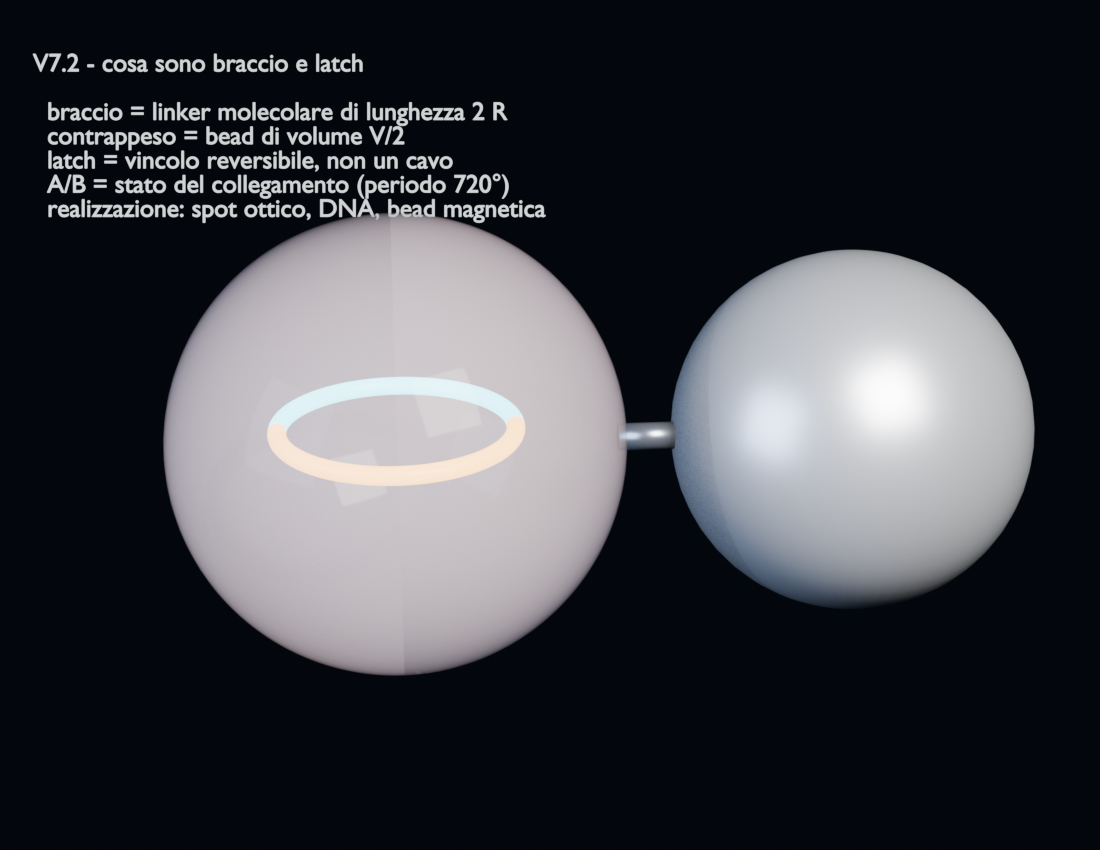
\includegraphics[width=0.78\textwidth]{../blender/v72_latch.png}
\caption{Primo piano: linker, bead e indicatore A/B. I cavi della scena
principale sono un diagramma del collegamento topologico, non un meccanismo
letterale.}
\label{fig:latch}
\end{figure}

\subsection{La firma del 720$^\circ$}

Se il latch scambia A e B a 360$^\circ$ e li riporta a 720$^\circ$, allora
$s(\theta+2\pi)=-s(\theta)$. L'orientazione è 360$^\circ$-periodica; lo stato
è 720$^\circ$-periodico. In frequenza, $\omega$ ha una riga a
$f_{\rm rot}=\omega/(2\pi)$; $s$ ha la fondamentale a
$f_{\rm rot}/2=\omega/(4\pi)$. La Figura~\ref{fig:firma} mostra i due spettri.
Questa distinzione è il contenuto fisico del 720$^\circ$; senza un
osservabile dispari sotto 360$^\circ$ non c'è nessun subarmonico da misurare.

\begin{figure}[H]
\centering
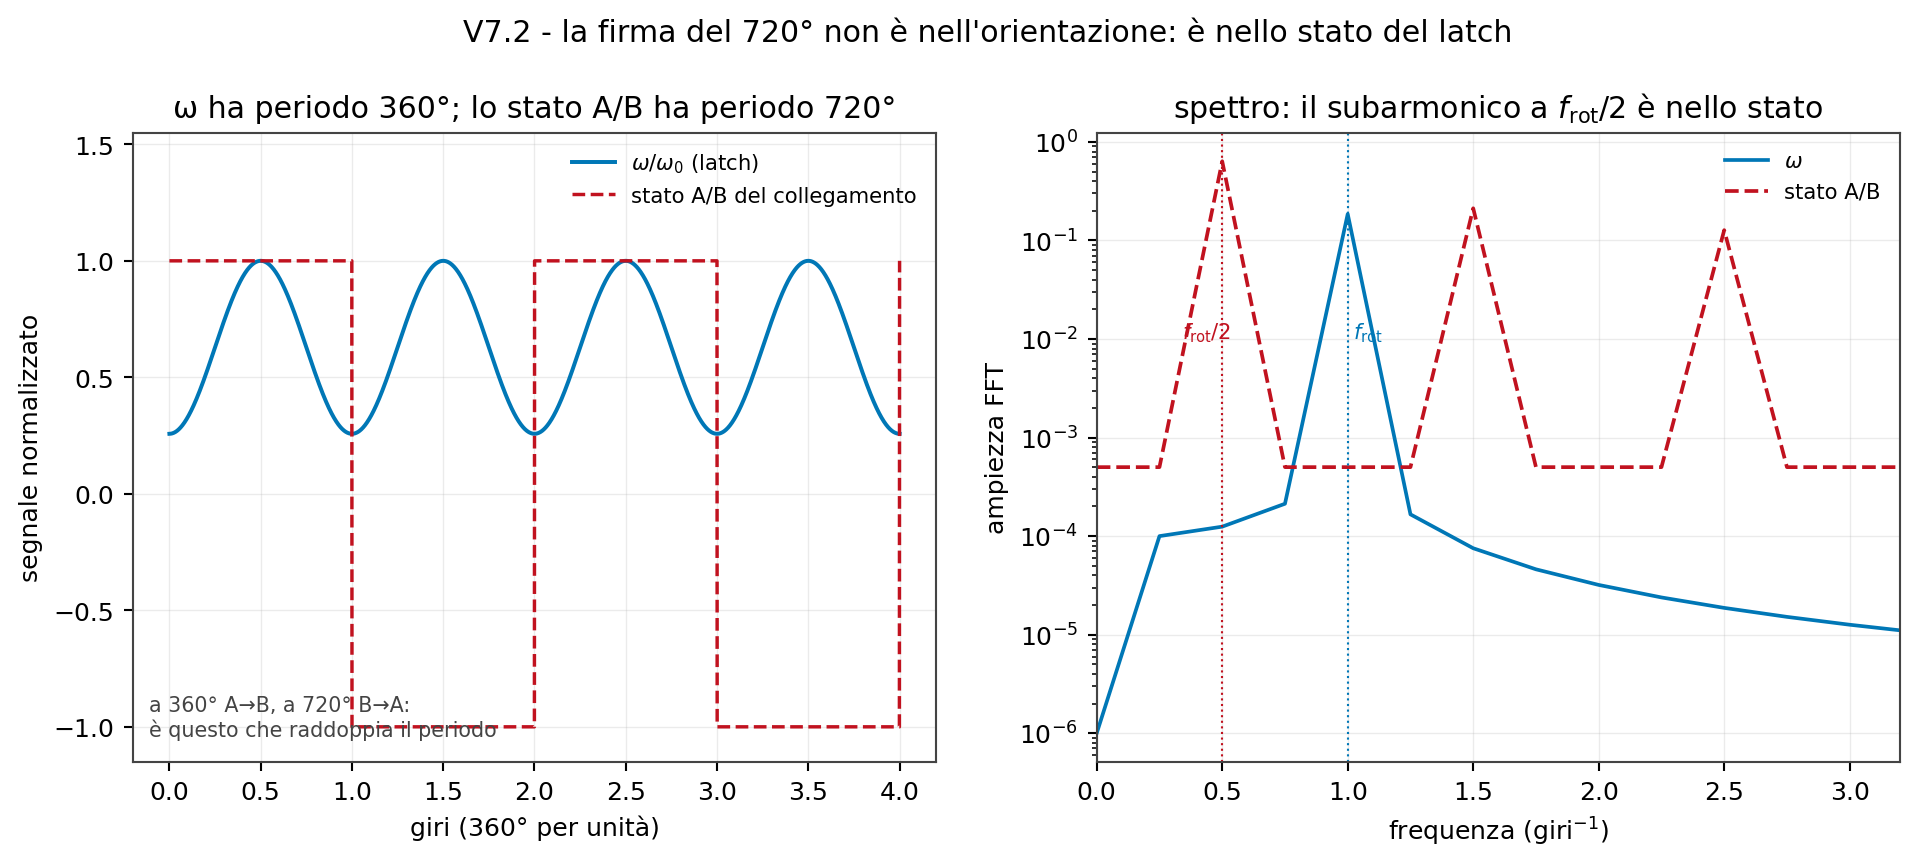
\includegraphics[width=\textwidth]{../figure/fig_V72_firma.png}
\caption{A sinistra $\omega$ (periodo 360$^\circ$) e lo stato A/B (periodo
720$^\circ$). A destra i due spettri: la riga a $f_{\rm rot}$ è la rotazione,
quella a $f_{\rm rot}/2$ è lo stato del latch.}
\label{fig:firma}
\end{figure}

\section{La firma misurabile e il rumore}
\label{sec:rumore}

\subsection{La curva deterministica non è quello che si misura}

La V7.1 disegnava la modulazione di $\omega$ come una sinusoide pulita. A
$Pe_r=10$ il moto è orientato, ma la fluttuazione istantanea è grande. Il
coefficiente di diffusione rotazionale è
\begin{equation}
D_r=\frac{kT}{\beta_{\rm tot}},\qquad
\tau_r=\frac{1}{2D_r}=\frac{\beta_{\rm tot}}{2kT}.
\end{equation}
A $R=0.3\,\micro$m, $\beta_{\rm tot}=1.05\times10^{-20}$\,N\,m\,s,
$D_r\approx0.99$\,rad$^2$/s, $\tau_r\approx0.5$\,s. La diffusione angolare
per un giro è
\begin{equation}
\sigma_\theta(360^\circ)=\sqrt{2D_rT_{360}}\approx1.39\,\text{rad}
\approx80^\circ,
\end{equation}
indipendente da $R$ a $Pe_r$ fissato. La traccia di $\omega$ è quindi
dominata dal rumore; la media ripiegata su $\theta$ recupera la modulazione.
La Figura~\ref{fig:rumore} mostra la traccia, la media e lo spettro.

\begin{figure}[H]
\centering
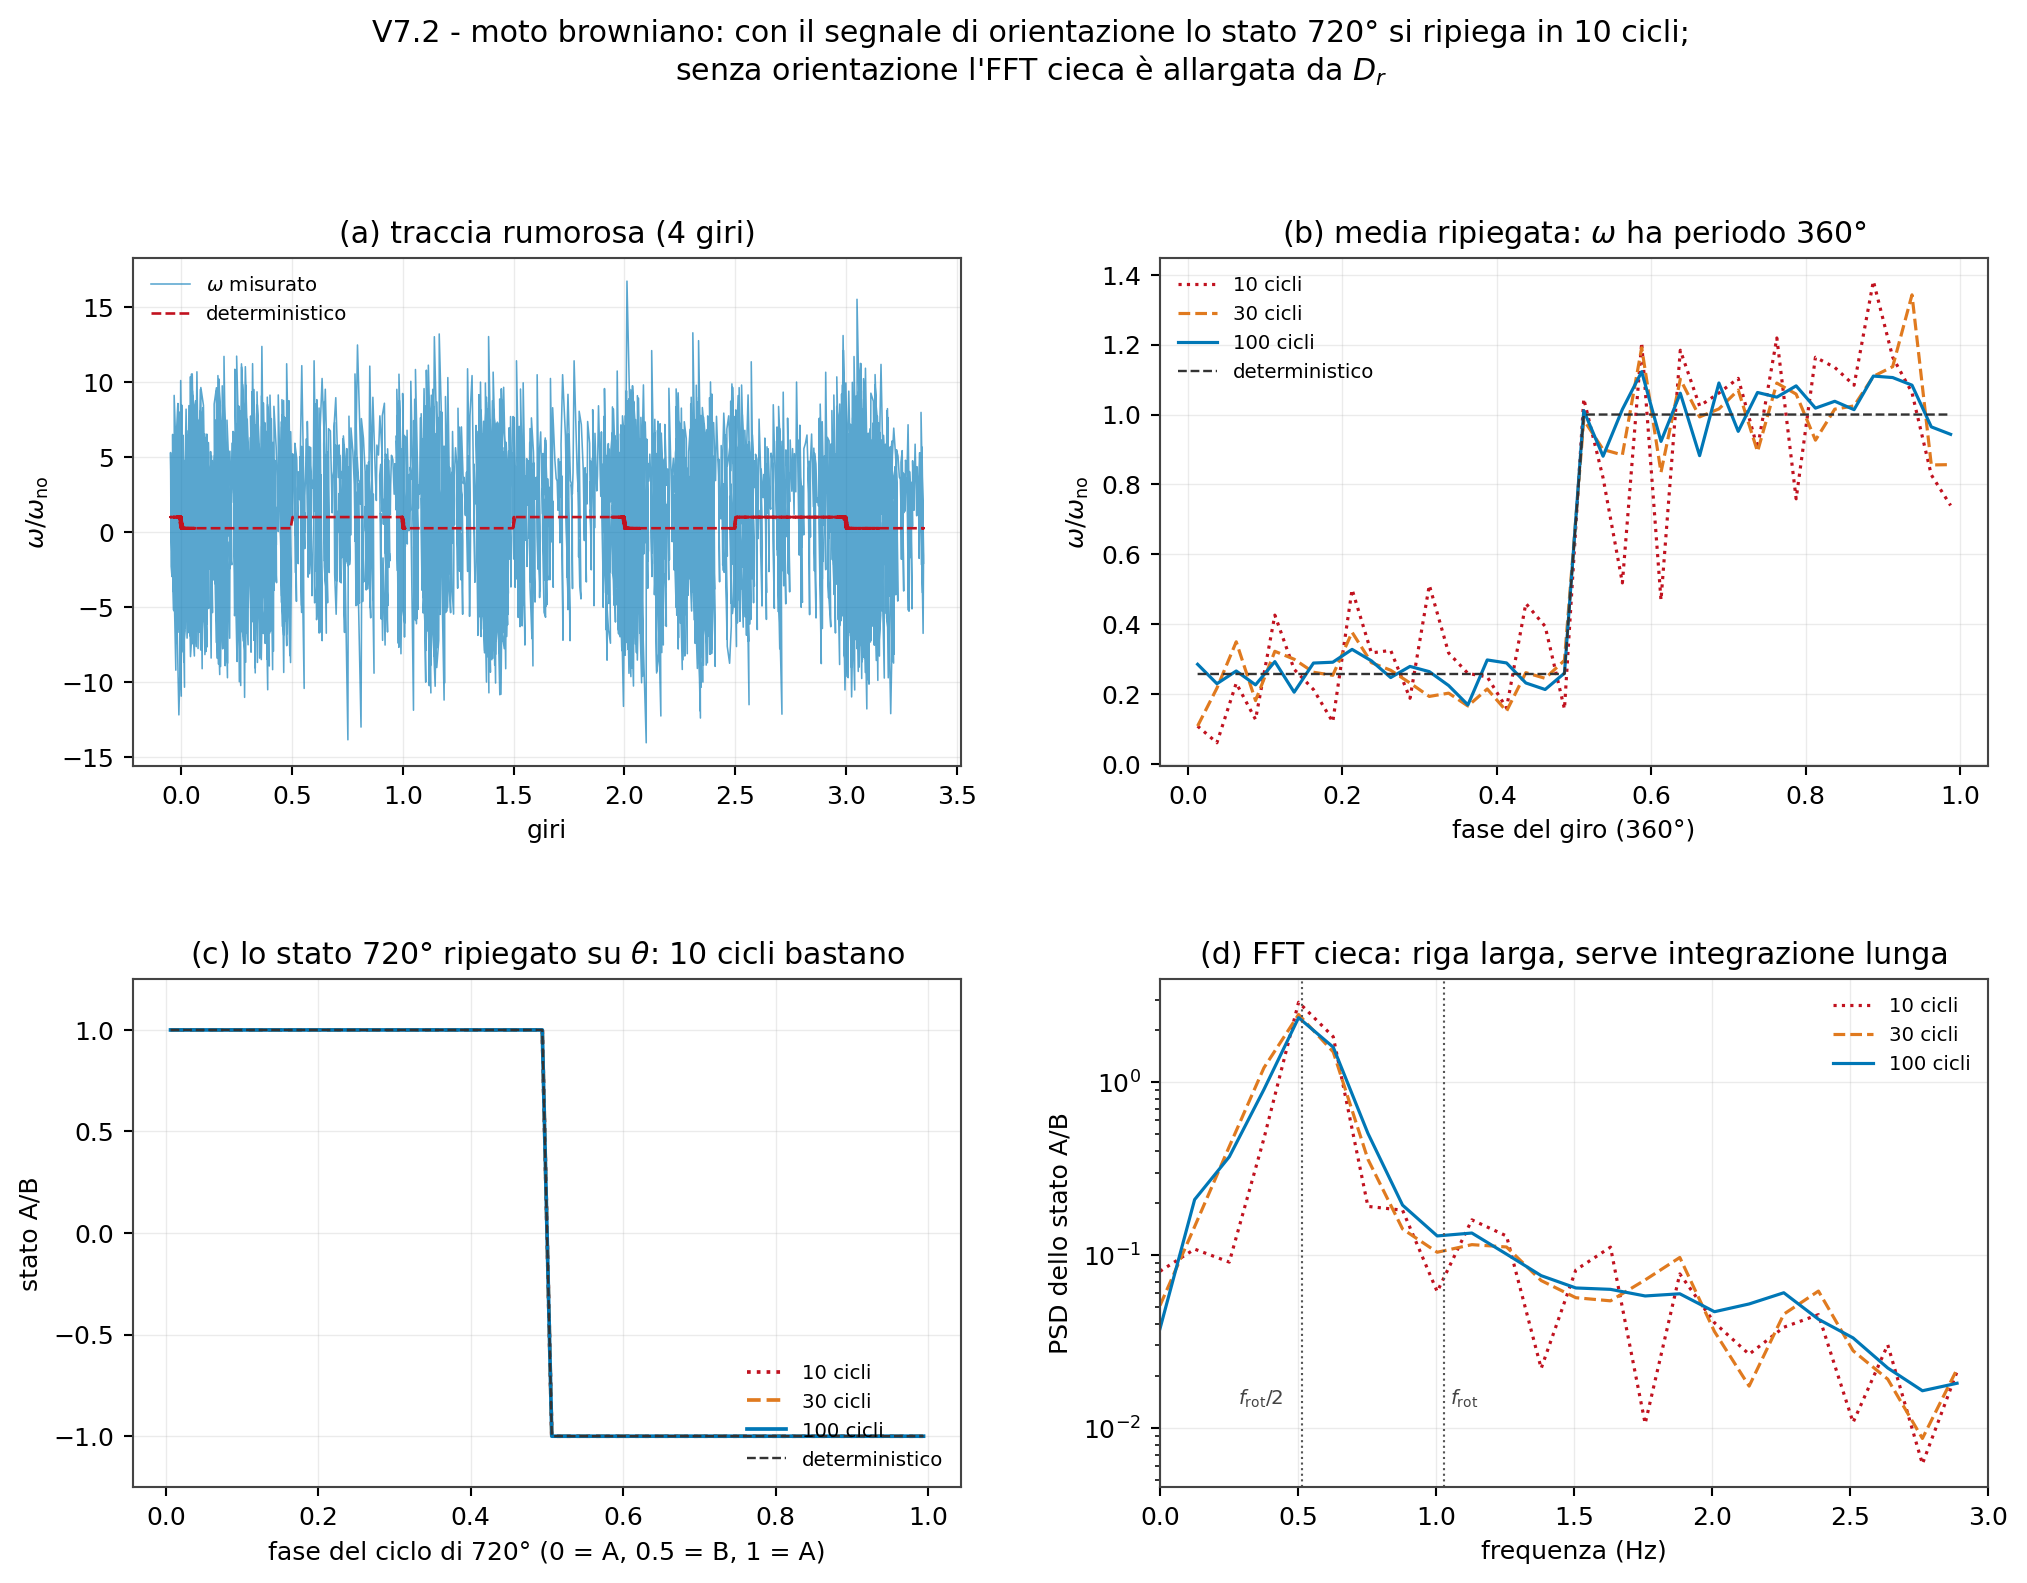
\includegraphics[width=\textwidth]{../figure/fig_V72_rumore.png}
\caption{Simulazione di Langevin per $R=0.3\,\micro$m, 200 cicli. (a) la
traccia è rumorosa; (b) la media ripiegata su $\theta$ recupera il periodo
360$^\circ$ di $\omega$; (c) lo stato 720$^\circ$ si ripiega su $\theta$ in
10 cicli; (d) l'FFT cieca è allargata da $D_r$ e richiede integrazione lunga.}
\label{fig:rumore}
\end{figure}

\subsection{Quanti cicli servono}

Ci sono due protocolli, con due risposte diverse.

\textbf{Con il segnale di orientazione.} Si misura $\theta(t)$ e il segnale
A/B $s(t)$; si ripiega $s$ su $\theta\bmod4\pi$. Poiché $s$ è una funzione
di $\theta$, la diffusione browniana non sposta la fase relativa: 10 cicli
bastano per vedere il quadrato A/B. La curva (c) della
Figura~\ref{fig:rumore} lo mostra. Questo è il protocollo consigliato.

\textbf{Con la sola FFT cieca.} Se non si ha $\theta$, la riga a
$f_{\rm rot}/2$ è allargata da $D_r$ e il numero di cicli cresce. La
Tabella~\ref{tab:rumore} dà la stima per SNR$=10$: circa 120 cicli con 20
bin per ciclo, circa 600 con 100 bin per ciclo. A $R=0.3\,\micro$m,
$T_{720}\approx1.94$\,s, quindi 120 cicli sono $\sim4$ minuti e 600 cicli
sono $\sim19$ minuti. A $R=1\,\micro$m i tempi crescono come $R^3$: 72\,s per
ciclo, cioè ore. Il confronto con la V7.1 è netto: la ``firma'' non è
un'osservazione visiva, è un protocollo di acquisizione e analisi.

\begin{table}[H]
\centering\small
\begin{tabular}{rrrrrrr}
\hline
$R$ & $D_r$ & $\tau_r$ & $\sigma_\theta(360^\circ)$ &
$N_{10}$ (20 bin) & $N_{10}$ (100 bin) & $T_{720}$ \\
\micro m & rad$^2$/s & s & deg & cicli & cicli & s \\
\hline
0.3 & 0.992 & 0.50 & 80 & 119 & 595 & 1.94 \\
0.5 & 0.214 & 2.33 & 80 & 119 & 595 & 9.00 \\
1.0 & 0.027 & 18.68 & 80 & 119 & 595 & 72.04 \\
\hline
\end{tabular}

\caption{Stima del numero di cicli per SNR$=10$ sulla modulazione di
$\omega$, a 800\,nm e $z=2\,\micro$m.}
\label{tab:rumore}
\end{table}

\subsection{La modulazione corretta}

La modulazione di $\omega$ è 74.2\,\% (Eq.~\ref{eq:modomega}), non 84.2\,\%.
L'84.2\,\% è la frazione di inerzia. La figura della V7.1 che usa 84.2\,\%
sovrastima l'ampiezza del segnale del 13\,\% relativo. La differenza non è
fatale, ma va corretta prima di confrontarsi con un esperimento.

\section{Limiti del mezzo continuo e del modello termico}
\label{sec:limiti}

\subsection{Il sangue non è newtoniano}

Il valore 4\,mPa\,s è quello ad alto shear. A $\omega\sim4$\,rad/s e con
$R<1\,\micro$m la viscosità effettiva può essere 10\,mPa\,s: $\beta$ e
$T_{720}$ raddoppiano, $E_{720}$ raddoppia. La Tabella~\ref{tab:viscosita}
mostra la sensibilità. $\Delta T$ non cambia, perché $P_{\rm target}$ non
dipende da $\mu$; cambia il tempo, quindi la dose. La finestra in $R$ resta
la stessa; la finestra operativa in \emph{tempo} si restringe.

\begin{table}[H]
\centering\small
\begin{tabular}{rrrrrrrl}
\hline
$R$ & $\mu$ & $T_{720}$ & $E_{720}$ & $\Delta T$ & $Re$ &
$\tau/\tau_B$ & sicuro \\
\micro m & mPa\,s & s & mJ & K & -- & -- & \\
\hline
0.3 & 4 & 1.9 & 1.4 & 12.3 & 9.7e-08 & 18.9 & solo op. \\
1.0 & 4 & 72.0 & 4.2 & 1.0 & 2.9e-08 & 0.5 & sì \\
0.3 & 7 & 3.4 & 2.4 & 12.3 & 3.2e-08 & 18.9 & solo op. \\
1.0 & 7 & 126.1 & 7.4 & 1.0 & 9.5e-09 & 0.5 & sì \\
0.3 & 10 & 4.9 & 3.4 & 12.3 & 1.6e-08 & 18.9 & solo op. \\
1.0 & 10 & 180.1 & 10.6 & 1.0 & 4.7e-09 & 0.5 & sì \\
\hline
\end{tabular}

\caption{Sensibilità alla viscosità, 800\,nm, $z=2\,\micro$m, latch a metà
ciclo. $\tau_B$ è la coppia di snervamento stimata con
$\sigma_y=0.01$\,Pa.}
\label{tab:viscosita}
\end{table}

\subsection{Il continuo scricchiola}

A $R=0.3\,\micro$m il rotore è più piccolo di un globulo rosso
(6--8\,$\micro$m di diametro). Stokes descrive una viscosità media, non
l'urto con le cellule. Il numero di Reynolds rotazionale è
$Re=\rho\omega R^2/\mu\sim10^{-7}$: l'inerzia del fluido è trascurabile, ma
il continuo non è garantito. A basso shear il sangue ha uno sforzo di
snervamento di circa 0.005--0.01\,Pa; la coppia ottica lo supera di un
fattore 20--40 a $R=0.3\,\micro$m, ma il transitorio di avvio va verificato.
La conclusione è che il valore 4\,mPa\,s è un valore di lavoro, non una
misura: la V7.2 lo tratta come parametro e riporta l'intervallo.

\subsection{La termica è una stima, non un certificato}

La formula usata per $\Delta T_{\rm path}$ è una sorgente lineare in mezzo
infinito:
\begin{equation}
\Delta T_{\rm path}=\frac{P_{\rm inc}-P_{\rm target}}
{2\pi\kappa z}\ln\frac{z}{w_0}.
\end{equation}
La perfusione (Pennes) ha una lunghezza
$L=\sqrt{\kappa/(\rho_bc_b\omega_b)}\approx1.4$\,cm per
$5$\,mL/100\,g/min. Su $2$--$100\,\micro$m il sink volumetrico è piccolo, ma
la parete del capillare e il flusso contano. La coagulazione locale aumenta
assorbimento e viscosità: il $\Delta T$ può peggiorare, non migliorare. La
stima va letta come ordine di grandezza; un modello Pennes con geometria del
vaso è il passo successivo.

\subsection{20 K non è una soglia di sicurezza}

310\,K + 20\,K = 330\,K = 57\,$^\circ$C: coagulazione. La soglia prudente
per esposizione prolungata è 5\,K (42\,$^\circ$C). Le celle ``valide'' della
V7.1 con $\Delta T=9$--$19$\,K sono già in ipertermia. Se il dispositivo
deve stare nel sangue, il criterio operativo è 5\,K, non 20\,K. Questo
sposta il punto di lavoro a $R\approx0.5$--$0.6\,\micro$m,
$T_{720}\approx7$--$12$\,s, $E_{720}\approx1.4$--$1.8$\,mJ. È un punto più
lento, ma è l'unico che non sta già scaldando il tessuto oltre la soglia di
sicurezza.

\section{Cosa resta da fare}
\label{sec:resta}

\begin{enumerate}\itemsep2pt
\item \textbf{Misurare la distribuzione di taglia.} Se il CV è $\ge15\,\%$,
il picco a 2.34\,$\micro$m non deve superare 20\,K. È il test più semplice
per validare o smentire la spiegazione degli zeri di forma.
\item \textbf{Misurare il latch.} Serve un tempo di risposta e una forza;
senza, il modello resta cinematico. Il test A/B è diretto: il segnale deve
avere periodo 720$^\circ$, non 360$^\circ$.
\item \textbf{Sangue intero in vitro.} Misurare $\mu_{\rm eff}$ a
$\omega\sim4$\,rad/s e il ruolo dello snervamento. Il valore 4\,mPa\,s va
sostituito con una misura, non con una nota.
\item \textbf{Mie completo.} Il canale a ritardo è trattato con
$\delta=2\pi\Delta n(2R)/\lambda$; una sfera reale ha risonanze
morfologiche. Un calcolo Mie/DDA direbbe se i picchi a 2.34 e
3.11\,$\micro$m sono davvero zeri di forma o risonanze.
\item \textbf{Pennes con geometria del vaso.} La stima lineare va sostituita
con un modello 2D/3D che includa parete, flusso e perfusione.
\item \textbf{Protocollo di falsificazione.} Se il segnale A/B ha periodo
360$^\circ$, la topologia non c'è. Se il subarmonico a $f_{\rm rot}/2$ non
emerge dopo 600 cicli, il latch non è accoppiato. Se il picco a
2.34\,$\micro$m resta sopra 20\,K con CV$\ge15\,\%$, la spiegazione di forma
è sbagliata.
\end{enumerate}

\section*{Codice, dati e riproducibilità}
\addcontentsline{toc}{section}{Codice, dati e riproducibilità}

Ogni numero del testo viene da un file generato dal codice accluso. La
cartella \texttt{versione 7.2} contiene:

\begin{center}\small
\begin{tabular}{p{3.6cm}p{10.0cm}}
\hline
file & funzione \\
\hline
\texttt{v72\_contrappeso.py} & griglia 532/800/1064\,nm, costo energetico,
rumore, viscosità, latch \\
\texttt{v72\_figure.py} & figure \texttt{fig\_V72\_*.png} \\
\texttt{v72\_rumore.py} & simulazione di Langevin e figura del rumore \\
\texttt{v72\_tabelle.py} & tabelle LaTeX da \texttt{V72\_sintesi.json} \\
\texttt{v72\_blender.py} & scena e render \texttt{v72\_*.png} \\
\hline
\end{tabular}
\end{center}

I dati sono in \texttt{dati/V72\_griglia.json},
\texttt{dati/V72\_sintesi.json} e \texttt{dati/V72\_rumore.json}. Le figure
sono in \texttt{figure/}, i render in \texttt{blender/}, le tabelle in
\texttt{tabelle/}. La V7.1 resta intatta: la V7.2 è una cartella separata.

\begin{thebibliography}{9}\small
\bibitem{friese1996} M. E. J. Friese, J. Enger, H. Rubinsztein-Dunlop,
N. R. Heckenberg, \emph{Optical angular-momentum transfer to trapped
absorbing particles}, Phys. Rev. A \textbf{54}, 1593 (1996).
\bibitem{friese1998} M. E. J. Friese, T. A. Nieminen, N. R. Heckenberg,
H. Rubinsztein-Dunlop, \emph{Optically driven micromachine elements},
Nature \textbf{394}, 348 (1998).
\bibitem{mie1908} G. Mie, \emph{Beiträge zur Optik trüber Medien, speziell
kolloidaler Metallösungen}, Ann. Phys. \textbf{330}, 377 (1908).
\bibitem{pennes1948} H. H. Pennes, \emph{Analysis of tissue and arterial
blood temperatures in the resting human forearm}, J. Appl. Physiol.
\textbf{1}, 93 (1948).
\bibitem{berg1993} H. C. Berg, \emph{Random Walks in Biology}, Princeton
University Press (1993).
\bibitem{purcell1977} E. M. Purcell, \emph{Life at low Reynolds number},
Am. J. Phys. \textbf{45}, 3 (1977).
\bibitem{lauga2009} E. Lauga, T. R. Powers, \emph{The hydrodynamics of
swimming microorganisms}, Rep. Prog. Phys. \textbf{72}, 096601 (2009).
\end{thebibliography}

\end{document}
